\documentclass[10pt, a4paper]{article}
\usepackage[latin1]{inputenc}
\usepackage{graphicx}
\usepackage[pdftex, linkbordercolor={0 0 1}]{hyperref}
\usepackage{float}
\usepackage{amsfonts}
\usepackage{lscape}
\pagestyle{empty}
\parindent0pt

\graphicspath{{images/}}

\newcommand{\req}[1]{\textsuperscript{(req. \ref{#1})}}
\newcommand{\reqdefLabel}[1]{\label{#1}}
\newcommand{\reqdef}[1]{\textbf{(see \ref{#1})}}
\newcommand{\saf}[1]{\emph{see also Figure \ref{fig: #1}}}

\begin{document}
\title{MiXiM - Physical Layer}
\author{Karl Wessel: wessel$@$tkn.tu-berlin.de\\
Michael Swigulski: swigulski$@$tkn.tu-berlin.de}
\date{20. November 2007}
\maketitle
%\section{Preamble}

\subsection{What is the Physical Layer}
TODO: write description

\section{requirement specification}
\label{req_spec}

\subsection{Overview}
\label{overview}

\begin{itemize}
 \item provide status information to MAC
 \item switch states (RX, TX, SLEEP)
 \item send packets to air/channel
 \item receive packets / listen for packets
 \item provide hooks for statistical information
 \item configurable settings
\end{itemize}

\subsection{provide status information to MAC}
\label{stateInfo}

In addition to received packets the physical layer has to provide some other information to the MAC layer.
Some of this information has to be provided passively\reqdefLabel{defprovpassive} on demand (e.g. current mode) and some should be delivered actively\reqdefLabel{defprovactive} to the MAC layer on certain events (e.g. transmission of a packet complete).

\noindent Information which has to be provided to MAC on demand:
\begin{itemize}
 \item channelstate: idle (boolean) or RSSI\reqdefLabel{defchannelstate}
 \item current mode (RX, TX, SLEEP)\reqdefLabel{defcurrentmode}
\end{itemize}

\noindent Information which has to be provided to MAC the moment it occurs:
\begin{itemize}
 \item transmission over (send)\reqdefLabel{deftxover}
\end{itemize}

\pagebreak
\subsection{switch states}
\label{switchstates}

The physical layer has to be able to switch between the following things:

\begin{itemize}
 \item current mode (RX, TX, SLEEP)\reqdefLabel{defswitchmode}
\end{itemize}

Switching from one mode to another may take some time. Whereas the switching time may depends to whitch mode we are switching.\reqdefLabel{defswitchtimes}

\begin{figure}[t]
 \centering
 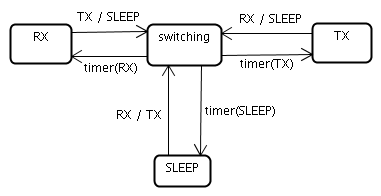
\includegraphics[width=240pt]{req_spec/stateMachineMode.png}
 % stateMachineMode.png: 1179666x1179666 pixel, 0dpi, infxinf cm, bb=
 \caption{State machine for current mode}
 \label{fig: mode state machine}
\end{figure}

\pagebreak
\subsection{send packets}
\label{sendPackets}

The physical layer has to be able to send packets from the MAC 
Layer to the channel. 
We also want to support the possibility to control
the sending process after it has been started.\reqdefLabel{defsendControl}.

Before we can send packets the following things have to be 
assured:
\linebreak
\begin{itemize}
 \item the radio has to be in TX mode\reqdefLabel{defsendPreqMode}
 \item we are not already sending\reqdefLabel{defsendPreqSending}
 \item the channel should be idle (this is no hard requirement)\reqdefLabel{defsendPreqIdle}
\end{itemize}

The above items should be controlled by the MAC layer so the physical layer 
would only throw an error if they are not set.

The following information has to be attached by the MAC layer to the packet:

\begin{itemize}
 \item header bitrate\reqdefLabel{defsendCtrlHeaderBitrate}
 \item payload bitrate\reqdefLabel{defsendCtrlBitrate}
 \item channel\reqdefLabel{defsendCtrlChannel}
 \item TX power\reqdefLabel{defsendCtrlTXPower}
 \item size of packet\reqdefLabel{defsendCtrlSize}
\end{itemize}


The sending process itself is made up of the following steps:

\begin{enumerate}\reqdefLabel{defpacketFromMac}\reqdefLabel{defsendInfoTXPower}\reqdefLabel{deftxover2}\reqdefLabel{defsendToChannel}
 \item MAC layer gives packet and control info to physical layer
 \item check requirements for sending, throw error if they are not fulfilled
 \item add information needed by the receiving physical layer to packet (see below)
 \item add signal function transmission power\footnote{The receiver converts the same signal to receiving power over time.} over time)\footnote{The signal function could be more dimensional. E.g.: receiving power over time and channel.} to packet
 \item packet is send to channel by physical layer
 \item schedule transmission over message for MAC layer
\end{enumerate}

The following information is needed by the receiving physical layer:

\begin{itemize}
\item TX power (represented by the signal function)
\item position, move direction and speed of the sending host\reqdefLabel{defsendInfoMove}
\item the channel\reqdefLabel{defsendInfoChannel}
\item size of packet\reqdefLabel{defsendInfoSize}
\item the duration the signal would need to be transmitted\reqdefLabel{defsendInfoDuration}
\item the duration of the preamble\reqdefLabel{defsendInfoPreambleDuration}
\item the bitrate (payload and header)\reqdefLabel{defsendInfoBitrate}
\end{itemize}

\subsection{receive packets}
\label{receivePackets}

Because the packets arrive immediatly at every receiving node we have to simulate the receiving process:

\begin{enumerate}\reqdefLabel{defrcvSimDelay}\reqdefLabel{defrcvSimPreamble}\reqdefLabel{defrcvSimDuration}
\item simulate propagation delay (if needed)
\item simulate preamble duration
\item simulate payload duration
\end{enumerate}

We also have to simulate the attenuation of the signal strength\reqdefLabel{defrcvSimAttenuation}. This should be done by filtering the with the \textit{analogue models}.

If the preamble is transmitted the packet has to be classified as \textit{signal} or \textit{noise}\reqdefLabel{defrcvClassify}. The decision is made by the \textit{decider}. Therefore the preamble has to be filtered previously by the analogue models.\reqdefLabel{defrcvFilterPreamble}

If the transmission of a \textit{signal} is over we have to decide if it was received correctly.\reqdefLabel{defrcvIsCorrect} This is also done by the \textit{decider} by evaluating the \textit{signal to noise ratio} short \textit{SNR}. Of course we have to apply the \textit{analogue model} to the signal and every noise interfering with the signal beforehand.\reqdefLabel{defrcvFilterSignals} If the signal was received correctly we pass it to the MAC Layer.\reqdefLabel{defrcvPassToMAC}

\subsubsection{the analogue model}
\label{analogueModel}

The \textit{analogue model} simulates the attenuation of the signal strength by filtering the receiving power function\reqdefLabel{defanalogueFilter}.

There should be models to simulate the following things:

\begin{itemize}
 \item pathloss\reqdefLabel{defanalogueSimPathloss}
 \item shadowing\reqdefLabel{defanalogueSimShadowing}
 \item fading\reqdefLabel{defanalogueSimFading}
\end{itemize}

Further we set the following requirements to the \textit{analogue models}:

\begin{itemize}
 \item physical layer should be able to apply multiple \textit{analogue models} to a signal\reqdefLabel{defanalogueMulti}
 \item you should be able to set the \textit{analogue models} independent from physical layer\reqdefLabel{defanalogueIndependent}
 \item you should be able to add your own \textit{analogue models}\reqdefLabel{defanalogueExtensible}
\end{itemize}

\subsubsection{the decider}
\label{decider}

As mentioned already above the \textit{decider} has to decide the following things:

\begin{itemize}
\item classify packet as signal or noise at base of the preamble\reqdefLabel{defrcvClassify2}
\item decide if a packet was received correct at base of the signal at interfering noise\reqdefLabel{defrcvIsCorrect2}
\end{itemize}

We set the following requirements to the \textit{decider}:

\begin{itemize}
 \item you should be able to set the \textit{decider} independent from physical layer\reqdefLabel{defdeciderIndependent}
 \item you should be able to add your own \textit{decider}\reqdefLabel{defdeciderExtensible}
 \item the \textit{decider} should be able to return bitwise correctness of the \textit{signal} (on demand)\reqdefLabel{defdeciderBitwise}
\end{itemize}


\subsection{statistical information}
\label{statistic}

You should be able to get the following statistical information (the physical layer should not evaluate them but has to provide access to the according information):

\begin{itemize}
\item packet count\reqdefLabel{defstatPackets}
\item received signal strength\reqdefLabel{defstatRSS}
\item signal to noise ratio\reqdefLabel{defstatSNR}
\item bit error ratio\reqdefLabel{defstatBER}
\item collisions\reqdefLabel{defstatColls}
\end{itemize}

\subsection{parameters}
\label{parameters}

The following parameters of the physical layer should be freely configurable:

\begin{itemize}
	\item simulate propagation delay? (boolean)\reqdefLabel{defconfDelay}
	\item which analogue models should be used\reqdefLabel{defconfAnalogue}
	\item the parameters for the analogue models\reqdefLabel{defconfAnalogueParam}
	\item which decider should be used\reqdefLabel{defconfDecider}
	\item the parameters for the decider\reqdefLabel{defconfDeciderParam}
	\item thermal noise\reqdefLabel{defconfNoise}
	\item sensitivity\reqdefLabel{defconfSens}
	\item maximum TX power\reqdefLabel{defconfMaxTXPower}
	\item switching times between modes (RX, TX, SLEEP)\reqdefLabel{defconfSwitchingTimes}
\end{itemize}

\subsection{list of requirements}
\label{requirements}

\begin{enumerate}
 \item provide status information to MAC
	\begin{enumerate}
	\item provide passive (on demand) \reqdef{defprovpassive}\label{provpassive}
	\item provide active (messages) \reqdef{defprovactive}\label{provactive}
	\item channelstate: idle (boolean) or RSSI \reqdef{defchannelstate}\label{channelstate}
	\item current mode (RX, TX, SLEEP) \reqdef{defcurrentmode}\label{currentmode}
	\item transmission over event (send) \reqdef{deftxover} and \reqdef{deftxover2}\label{txover}
	\end{enumerate}
 \item switch states (RX, TX, SLEEP)
	\begin{enumerate}
	\item current mode \reqdef{defswitchmode}\label{switchmode}
	\item switching times \reqdef{defswitchtimes}\label{switchtimes}
	\end{enumerate}
 \item send packets to air/channel
	\begin{enumerate}
	\item get packet from MAC layer \reqdef{defpacketFromMac}\label{packetFromMac}
	\item control sending process \reqdef{defsendControl}\label{sendControl}
	\item control information needed from MAC
		\begin{enumerate}
		\item header bitrate \reqdef{defsendCtrlHeaderBitrate}\label{sendCtrlHeaderBitrate}
		\item payload bitrate \reqdef{defsendCtrlBitrate}\label{sendCtrlBitrate}
		\item channel \reqdef{defsendCtrlChannel}\label{sendCtrlChannel}
		\item TX power \reqdef{defsendCtrlTXPower}\label{sendCtrlTXPower}
		\item size of packet \reqdef{defsendCtrlSize}\label{sendCtrlSize}
		\end{enumerate}
	\item prerequirements
		\begin{enumerate}
		\item are in TX mode \reqdef{defsendPreqMode}\label{sendPreqMode}
		\item not already sending \reqdef{defsendPreqSending}\label{sendPreqSending}
		\item channel is idle \reqdef{defsendPreqIdle}\label{sendPreqIdle}		
		\end{enumerate}
	\item attach informations for receiver
		\begin{enumerate}
		\item attach transmission power over time function \reqdef{defsendInfoTXPower}\label{sendInfoTXPower}
		\item position, move direction and speed of the sending host \reqdef{defsendInfoMove}\label{sendInfoMove}
		\item channel \reqdef{defsendInfoChannel}\label{sendInfoChannel}
		\item size of packet \reqdef{defsendInfoSize}\label{sendInfoSize}
		\item duration \reqdef{defsendInfoDuration}\label{sendInfoDuration}
		\item duration of preamble \reqdef{defsendInfoPreambleDuration}\label{sendInfoPreambleDuration}
		\item bitrate (payload and header) \reqdef{defsendInfoBitrate}\label{sendInfoBitrate}
		\end{enumerate}	
	\item send to channel \reqdef{defsendToChannel}\label{sendToChannel}
	
	\end{enumerate}
 \item receive packets / listen for packets
		\begin{enumerate}
		\item simulate propagation delay \reqdef{defrcvSimDelay}\label{rcvSimDelay}
		\item simulate preamble \reqdef{defrcvSimPreamble}\label{rcvSimPreamble}
		\item simulate transmission duration \reqdef{defrcvSimDuration}\label{rcvSimDuration}
		\item simulate attenuation \reqdef{defrcvSimAttenuation}\label{rcvSimAttenuation}
		\item filter preamble \reqdef{defrcvFilterPreamble}\label{rcvFilterPreamble}
		\item filter signal and interfering noise \reqdef{defrcvFilterSignals}\label{rcvFilterSignals}
		\item pass correct packets to MAC \reqdef{defrcvPassToMAC}\label{rcvPassToMAC}
		\item analogue model
			\begin{enumerate}
			\item filter signal strength \reqdef{defanalogueFilter}\label{analogueFilter}
			\item simulate pathloss \reqdef{defanalogueSimPathloss}\label{analogueSimPathloss}
			\item simulate shadowing \reqdef{defanalogueSimShadowing}\label{analogueSimShadowing}
			\item simulate fading \reqdef{defanalogueSimFading}\label{analogueSimFading}
			\item more than one analogue model per phy \reqdef{defanalogueMulti}\label{analogueMulti}
			\item can be set independent from phy \reqdef{defanalogueIndependent}\label{analogueIndependent}
			\item can add own analogue models \reqdef{defanalogueExtensible}\label{analogueExtensible}
			\end{enumerate}
		\end{enumerate}
		\item decider
			\begin{enumerate}
			\item classify preamble as noise or signal \reqdef{defrcvClassify} and \reqdef{defrcvClassify2}\label{rcvClassify}
			\item decide if packet was received correct \reqdef{defrcvIsCorrect}\label{rcvIsCorrect}
			\item can be set independent from phy \reqdef{defdeciderIndependent}\label{deciderIndependent}
			\item can add own decider \reqdef{defdeciderExtensible}\label{deciderExtensible}
			\item return bitwise errors \reqdef{defdeciderBitwise}\label{deciderBitwise}
			\end{enumerate}
 \item provide hooks for statistical information
	\begin{enumerate}
	\item packet count \reqdef{defstatPackets}\label{statPackets}
	\item received signal \reqdef{defstatRSS}strength \label{statRSS}
	\item signal to noise ratio \reqdef{defstatSNR}\label{statSNR}
	\item bit error ratio \reqdef{defstatBER}\label{statBER}
	\item collisions \reqdef{defstatColls}\label{statColls}
	\end{enumerate}
 \item configurable settings
	\begin{enumerate}
	\item simulate propagation delay? (boolean) \reqdef{defconfDelay}\label{confDelay}
	\item which analogue models should be used \reqdef{defconfAnalogue}\label{confAnalogue}
	\item the parameters for the analogue models \reqdef{defconfAnalogueParam}\label{confAnalogueParam}
	\item which decider should be used \reqdef{defconfDecider}\label{confDecider}
	\item the parameters for the decider \reqdef{defconfDeciderParam}\label{confDeciderParam}
	\item thermal noise \reqdef{defconfNoise}\label{confNoise}
	\item sensitivity \reqdef{defconfSens}\label{confSens}
	\item maximum TX power \reqdef{defconfMaxTXPower}\label{confMaxTXPower}
	\item switching times between modes (RX, TX, SLEEP) \reqdef{defconfSwitchingTimes}\label{confSwitchingTimes}
	\end{enumerate}
\end{enumerate}



%\newcommand{\h}[1]{\textit{#1}}
\newcommand{\bp}{BasePhyLayer}
\newcommand{\bm}{BaseMacLayer}


\section{modelling}

\emph{Note: }We denote a Layer in a general meaning by 'Phy-Layer' 
or 'MAC-Layer' and our concrete C++ classes by \h{\bp} or \h{\bm}.


\subsection{overview}

Here we present the design- and interface details of the OMNeT-module 
\h{\bp} to meet the requirement specification. That includes:

\begin{enumerate}
 \item internal class diagram of \h{\bp} and relation to \h{\bm}
 \item interface description for all involved C++ classes
 \item flow charts for reception of MacPacket from upper layer and 
 AirFrame from the channel
 \item some detailed flow charts for important sub processes
\end{enumerate}


\subsection{classgraph}

We start with the classgraph for the OMNeT-module \h{\bp} that shows 
its C++ classes, relations to other OMNeT-modules (especially \h{\bm})
and the OMNeT-messages sent between them.

The \h{\bp} holds a list\req{analogueMulti} of AnalogueModels and a pointer to a Decider. Thus the AnalogueModel and the Decider are submodules of \h{\bp}. This way one is able to change\req{analogueExtensible}\req{deciderExtensible} and replace\req{analogueIndependent}\req{deciderIndependent} them independently from the \h{\bp}.

\begin{figure}[H]
 \centering
 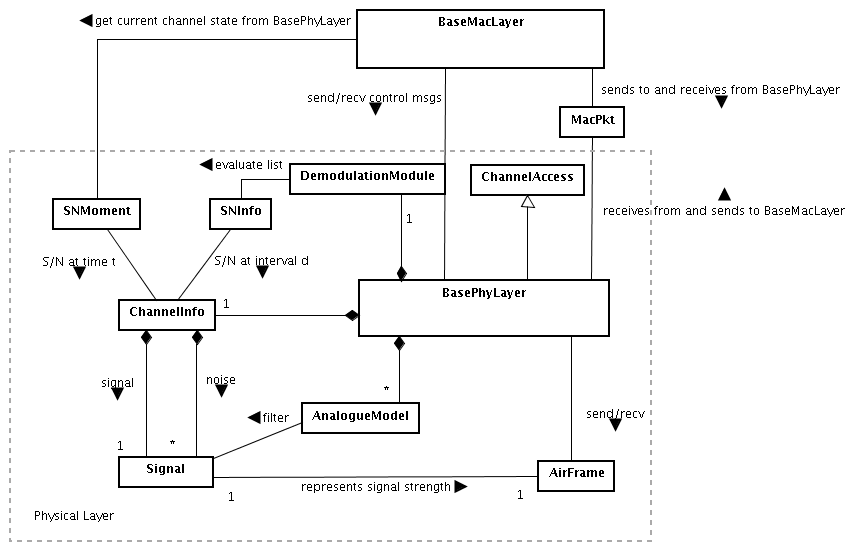
\includegraphics[width = \textwidth]{modelling/class_diagram.png}
 \caption{class graph}
 \label{fig: classgraph}
\end{figure}


\subsection{The \h{\bp} interface}

In this section we focus on how one is able to communicate with the 
\h{\bp}, i.e. especially the \h{\bm} which is connected to the \h{\bp}
in three ways:

\begin{enumerate}
 \item OMNet-channel for data messages
 \item OMNet-channel for control messages
 \item a reference to \h{\bp}.
\end{enumerate} 

The data channel is used to send and receive\req{packetFromMac} MacPkts to and from the \h{\bp}.

The control channel is used by the \h{\bp} to inform the \h{\bm} about
certain events\req{provactive}, like the TX\_OVER\req{txover} message 
which indicates the end of a sending transmission.

The reference provides a passive way\req{provpassive} for the  \h{\bm} to  get information about the current channel state\req{channelstate} and to get\req{currentmode} and set\req{switchmode} the current mode (RX, TX, SLEEP).
Switching times\req{switchtimes} from one mode to another are controlled internaly by a state machine. \saf{mode state machine}.


\begin{figure}[H]
 \centering
 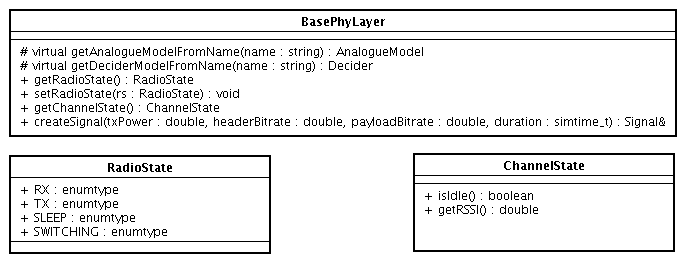
\includegraphics[width = \textwidth]{modelling/BasePhyLayer_members.png}
 \caption{BasePhyLayer interface}
 \label{fig: BasePhyLayer interface}
\end{figure}



\subsection{AnalogueModel and Signal}
\label{AM and Signal}

The Signal is designed one-dimensional (power-over-time) by default with a specified time point for start and end of the Signal. The owner is able
to add and request values at a specific time point\req{sendInfoTXPower}.
The Method getTimeIterator() returns an appropriate SignalTimeIterator needed for applying AnalogueModels to the Signal.

\begin{quote}
\emph{NOTE: Anyone who subclasses Signal should make shure to have a properly
working SignalTimeIterator (subclassed) for it. The SignalTimeIterator should always iterate over every time stamp in each dimension. This way simple AnalogueModels will be able to filter the Signal independent from its dimension.}
\end{quote}

Further the Signal is set the packets header and payload bitrate\req{sendInfoBitrate},  the Move of the Host\req{sendInfoMove}, the size of the packet\req{sendInfoSize} and the channel to send the packet to\req{sendInfoChannel} by \h{\bp}.

\emph{See also \ref{AirFrame and Signal}.}

\begin{figure}[H]
 \centering
 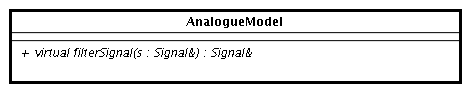
\includegraphics[width = \textwidth]{modelling/AnalogueModel_members.png}
 \caption{analogue model interface}
 \label{fig: analogue model interface}
\end{figure}

The AnalogueModel offers functionality to filter a referenced signal\req{analogueFilter} in a specified interval\req{rcvFilterSignals} (e.g. preamble\req{rcvFilterPreamble}) or at a single point in time.

Three basic AnalogueModel classes are foreseen to be plugged into Phy-Layer to simulate pathloss\req{analogueSimPathloss}, shadowing\req{analogueSimShadowing} and fading\req{analogueSimFading}.\\
\h{\bp} is designed to apply an arbitrary number of AnalogueModels to a Signal.

\begin{figure}[H]
 \centering
 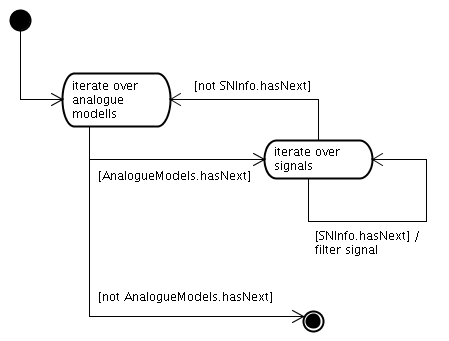
\includegraphics[width = 0.8\textwidth]{modelling/apply_analogue_modells_detail.png}%[width=300pt]
 \caption{application of analogue models}
 \label{fig: application analogue models}
\end{figure}



\subsection{SNInfo and ChannelInfo}

ChannelInfo keeps track of all AirFrames on the channel. It does not differentiate between \textit{signal} and \textit{noise}. \h{\bp} is able to
add and remove references to certain AirFrames to and from ChannelInfo.\\
ChannelInfo is able to record the whole channel over time from a start to a stop signal and can return a vector of Signals (references) that intersect with a given time interval.\\
SNInfo is created by \h{\bp} when a packet arrives to collect all signals from the channel that intersect with the reception time interval of the packet.

\begin{figure}[H]
 \centering
 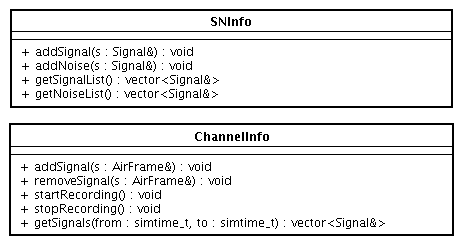
\includegraphics[width = \textwidth]{modelling/ChannelInfo_members.png}
 \caption{channel details}
 \label{fig: channel details}
\end{figure}




\subsection{Decider}

The Decider has two tasks:
\begin{enumerate}
	\item It decides whether we are able to receive a certain packet by evaluting
	the SNInfo for the packets preamble time interval, otherwise the packet will 	be considered noise\req{rcvClassify}
	\item When a packet has been received and is not noise the Decider 	returns a DeciderResult for that packet, that only contains if the packet was received correct or not correct by default\req{rcvIsCorrect}.
\end{enumerate}

A Decider that gives a richer DeciderResult (e.g. bitwise errors\req{deciderBitwise}) must be subclassed and implemented by the user.

\begin{figure}[H]
 \centering
 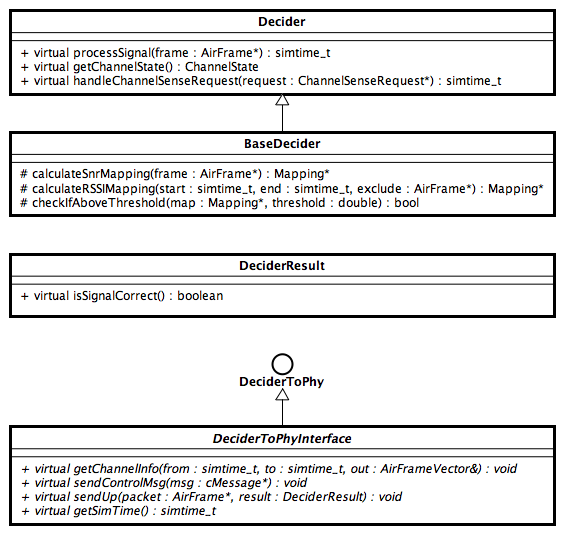
\includegraphics[width = \textwidth]{modelling/DeciderModule_members.png}
 \caption{Decider interface}
 \label{fig: Decider interface}
\end{figure}


\subsection{AirFrame}
\label{AirFrame and Signal}

AirFrame and Signal are both constructed by \h{\bp} with the help of MacToPhyControlInfo.
It is shown below how nessecary information for sending/receiving is distributed. Signal is already discussed in \ref{AM and Signal}.

\h{\bp} calculates duration\req{sendInfoDuration} and preamble duration\req{sendInfoPreambleDuration} of the packet and adds it to the AirFrame. 
To be able to control the sending process\req{sendControl} of another AirFrame every AirFrame has a unique id and a specific type which secifies if this is a normal AirFrame or a control-AirFrame.


\begin{figure}[H]
 \centering
 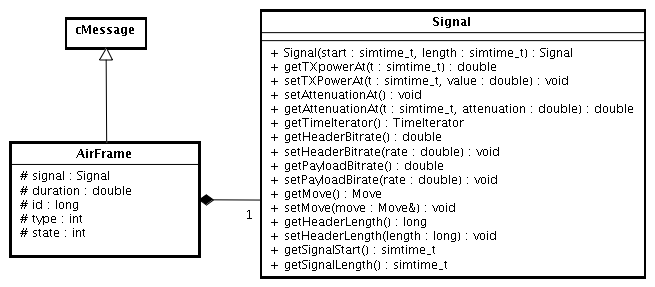
\includegraphics[width = \textwidth]{modelling/AirFrame_members.png}
 \caption{member arrangement in AirFrame and Signal}
 \label{fig: member AirFrame}
\end{figure}



\subsection{receiving a MacPkt}

On reception of a MacPkt from the MAC-Layer, \h{\bp} checks if:
\begin{enumerate}
	\item the radio is in TX mode\req{sendPreqMode},
	\item it is not already sending a packet\req{sendPreqSending} and
	\item the channel is idle\req{sendPreqIdle} (this is no hard requirement, \h{\bp} could send anyway).
\end{enumerate} 

If condition 1 or 2 is not fulfilled it will throw an error.\\

The MacToPhyControlInfo object attached to the MacPkt contains the information needed by \h{\bp} when constructing Signal and AirFrame to send to the channel. Right now it contains:

\begin{enumerate}
	\item the channel for sending\req{sendCtrlChannel},
	\item header bitrate\req{sendCtrlHeaderBitrate},
	\item payload bitrate\req{sendCtrlBitrate},
	\item TX Power\req{sendCtrlTXPower} and
	\item the size of the packet\req{sendCtrlSize}.

\end{enumerate}


\begin{figure}[H]
 \centering
 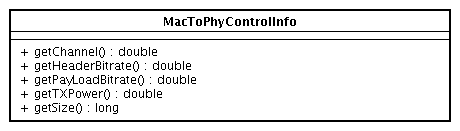
\includegraphics[width = \textwidth]{modelling/MacToPhyCtrlInfo_members.png}
 \caption{MacToPhyControlInfo interface}
 \label{fig: MacToPhyCtrlInfo interface}
\end{figure}

\h{\bp} is responsilbe for creating AirFrame and Signal and attaching information (parameters) to them. For detailed arrangement of information in Signal and AirFrame see \ref{AirFrame and Signal}.
When the AirFrame is complete and sent, \h{\bp} schedules a TX\_OVER message to the \h{\bm}(via control-message).

\begin{figure}[H]
 \centering
 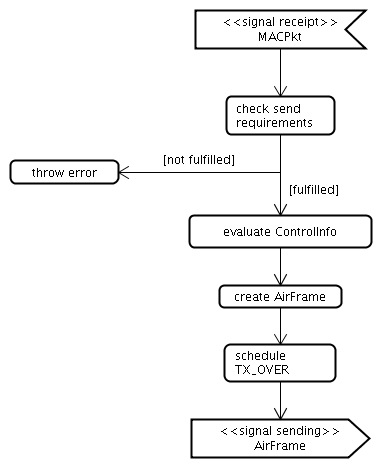
\includegraphics[width = 0.8\textwidth]{modelling/onMACPkt.png}
 \caption{sending process}
 \label{fig: sending process}
\end{figure}





\subsection{Receiving and processing an AirFrame}

The reception of an AirFrame is divided into:
\begin{enumerate}
	
	\item optional propagation delay\req{rcvSimDelay},
	\item reception of the preamble\req{rcvSimPreamble},
	\item application of AnalogueModels to the corresponding SNInfo\req{rcvSimAttenuation},
	\item decision whether packet is considered noise (Decider),
	\item reception of the packet\req{rcvSimDuration}.
\end{enumerate}

Afterwards the packet is either dropped (if considered noise) or processed. 

\begin{figure}[H]
 \centering
 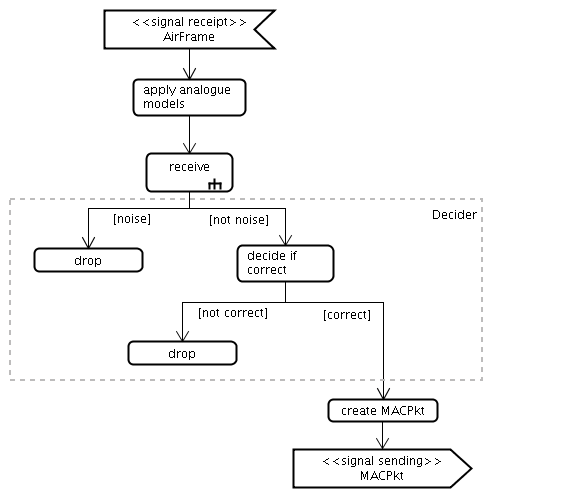
\includegraphics[width = 0.8\textwidth]{modelling/onAirFrame.png}
 \caption{receiving process}
 \label{fig: receiving process}
\end{figure}

The receiving process is modelled internally by a state machine that schedules the AirFrame that is received (since we have a pointer to it from the beginning) everytime a delay/time interval shall be simulated. That saves us the creation of additional self-messages.


\begin{figure}[H]
 \centering
 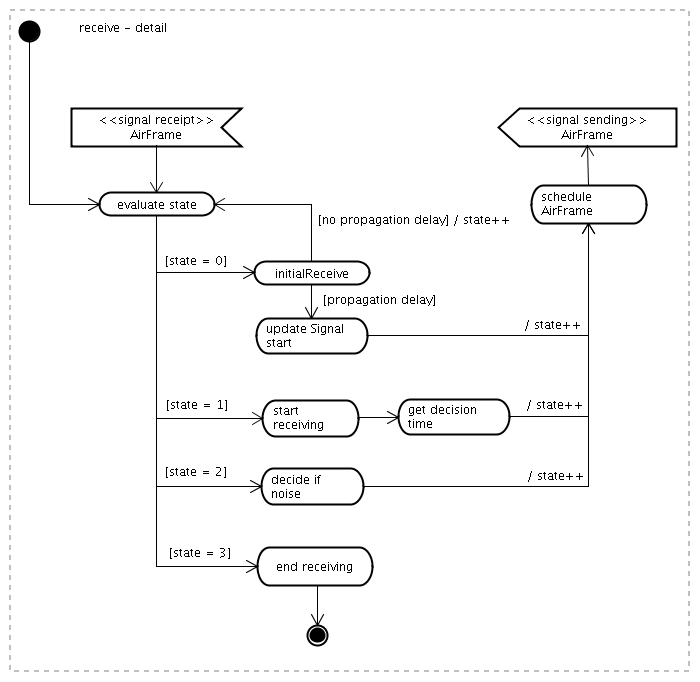
\includegraphics[width = \textwidth]{modelling/receive_detail.png}
 \caption{receive detail}
 \label{fig: receive detail}
\end{figure}

When the preamble of a packet is completely received, \h{\bp} constructs a SNInfo for the preamble, applies the AnalogueModels to it and passes it to the Decider to find out whether this packet is considered noise.

\begin{figure}[H]
 \centering
 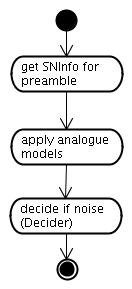
\includegraphics[width = 0.2\textwidth]{modelling/end_preamble_detail.png}
 \caption{end preamble detail}
 \label{fig: end preamble detail}
\end{figure}

In case a received packet is not \textit{noise} it is processed, i.e. \h{\bp} creates the corresponding SNInfo for the packet, applies AnalogueModels to it and passes the result to the Decider to check whether the packet was received correctly. If so, a MacPkt is created and handed up to Phy-Layer\req{rcvPassToMAC}.


\subsection{the .ned-file}

The .ned-file of the \h{\bp} has the following parameters:

\begin{itemize}
\item usePropagationDelay as \textit{boolean}\req{confDelay}
\item analogueModels as \textit{XML}\req{confAnalogue}\req{confAnalogueParam}
\item decider as \textit{XML}\req{confDecider}\req{confDeciderParam}
\item thermalNoise as \textit{numeric const}\req{confNoise}
\item sensitivity as \textit{numeric const}\req{confSens}
\item maximal TX power as \textit{numeric const}\req{confMaxTXPower}
\item switchTimeRX as \textit{numeric const}\req{confSwitchingTimes}
\item switchTimeTX as \textit{numeric const}\req{confSwitchingTimes}
\item switchTimeSleep as as \textit{numeric const}\req{confSwitchingTimes}
\end{itemize}

The parameters "analogueModels" and "decider" holds which analogueModels and decider to be used together with their parameters in XML formate. The exact formate still has to be declared!

%\subsection{provide status information to MAC}

%Passively provided information\req{provpassive}: \h{\bm} is equipped with a reference to \h{\bp} in order to obtain information
%about channelstate\req{channelstate} and current mode\req{currentmode} by
%simple method calls. \\
%Actively provided information\req{provactive}: A cMessage of the kind TX\_OVER
%is sent to MAC-Layer when a sending transmission is over\req{txover}, \saf{sending process}.



%\subsection{send packets}

%Since \h{\bm} has a reference to \h{\bp} it can obtain information about the mode the radio is is currently in\req{sendPreqMode}, it is not already sending to the channel on its own\req{sendPreqSending} and the channel is idle\req{sendPreqIdle} via method calls, \saf{BasePhyLayer interface}.

%The class MacToPhyControlInfo is designed as the container for control info\req{packetFromMac} the MAC-Layer
%wants to attach to the packet given down to Phy-Layer for sending.
%The packet itself is handed down as a MacPkt via OMNeT-channel. 

















\newcommand{\h}[1]{\textit{#1}}
\newcommand{\bp}{BasePhyLayer}
\newcommand{\bm}{BaseMacLayer}


\section{modelling}

\emph{Note: }We denote a Layer in a general meaning by 'physical layer' 
or 'MAC layer' and our concrete C++ classes by \h{\bp} or \h{\bm}.

\subsection{overview}

Here we present the design- and interface details of the OMNeT-module 
\h{\bp} to meet the requirement specification. That includes:

\begin{enumerate}
 \item internal class diagram of \h{\bp} and relation to \h{\bm}
 \item interface description for all involved C++ classes
 \item flow charts for reception of MacPacket from upper layer and 
 AirFrame from the channel
 \item some detailed flow charts for important sub processes
\end{enumerate}


\subsection{classgraph}

We start with the classgraph for the OMNeT-module \h{\bp} that shows 
its C++ classes, relations to other OMNeT-modules (especially \h{\bm})
and the OMNeT-messages sent between them.

The \h{\bp} holds a list\req{analogueMulti} of AnalogueModels and a pointer to a
Decider. Thus the AnalogueModel and the Decider are submodules of \h{\bp}. This
way one is able to change\req{analogueExtensible}\req{deciderExtensible} and
replace\req{analogueIndependent}\req{deciderIndependent} them independently from
the \h{\bp}.

\begin{figure}[H]
 \centering
 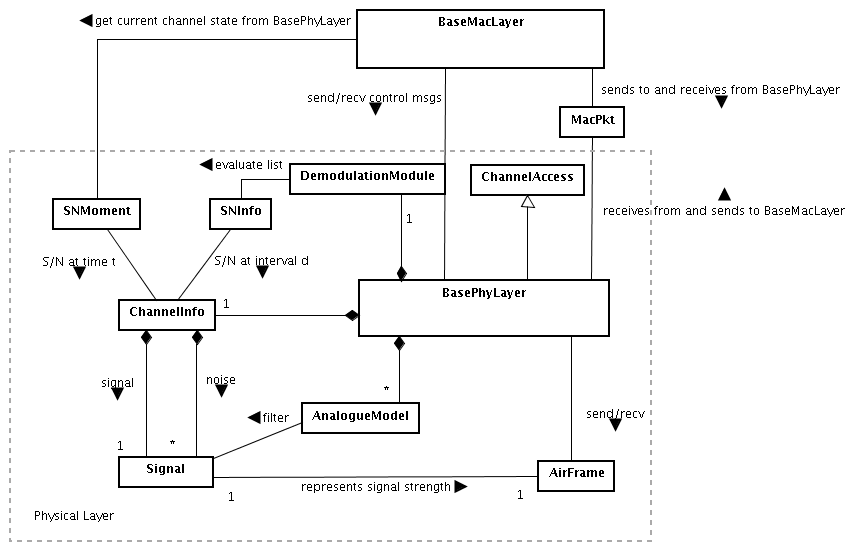
\includegraphics[width = \textwidth]{modelling/class_diagram.png}
 \caption{class graph}
 \label{fig: classgraph}
\end{figure}


\subsection{The \h{\bp} interface}

In this section we focus on how one is able to communicate with the 
\h{\bp}, i.e. especially the \h{\bm} which is connected to the \h{\bp}
in three ways:

\begin{enumerate}
 \item OMNeT-channel for data messages
 \item OMNeT-channel for control messages
 \item a reference to \h{\bp}.
\end{enumerate} 

The \underline{data channel} is used to send and receive\req{packetFromMac} MacPkts to and
from the \h{\bp}. An appropriate ControlInfo is attached to the packet by the sending layer. \saf{MacToPhyCtrlInfo interface}\\

The \underline{control channel} is used by the \h{\bp} to inform the \h{\bm} about
certain events\req{provactive}, like the TX\_OVER\req{txover} message 
which indicates the end of a sending transmission.

A ChannelSenseRequest can be sent over \underline{control channel} from \h{\bm} to \h{\bp}. It is handed to the Decider (several times) that attaches a ChannelState and finally sent back to \h{\bm}.
\begin{figure}[H]
 \centering
 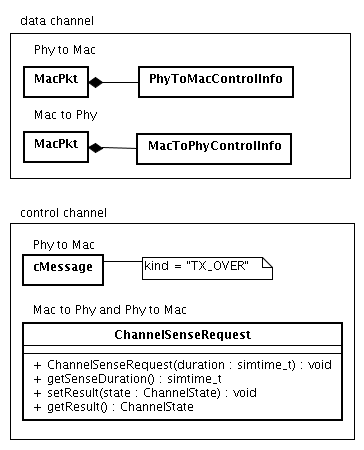
\includegraphics[width = 0.7\textwidth]{modelling/PhyMacMessages.png}
 \caption{messages sent between \h{\bp} an \h{\bm}}
 \label{fig: PhyMacMessages}
\end{figure}


The reference provides a passive way\req{provpassive} for the  \h{\bm} to  get
information about the current channel state\req{channelstate} (that is an alternative [immediate answer] to sending a ChannelSenseRequest) and to
get\req{currentmode} and set\req{switchmode} the current radiostate (RX, TX,
SLEEP).
Switching times\req{switchtimes} from one radio state to another are controlled
internally by a state machine. \saf{mode state machine}
\\

The createSignal method returns \h{\bm} a reference to a Signal at a minimum of necessary parameters, it only has to pass txPower, headerBitrate and payloadBitrate. This is the key method for \h{\bm} in order to create MacToPhyControlInfo properly.

% interface description here
\label{SignalCreation}

\begin{figure}[H]
 \centering
 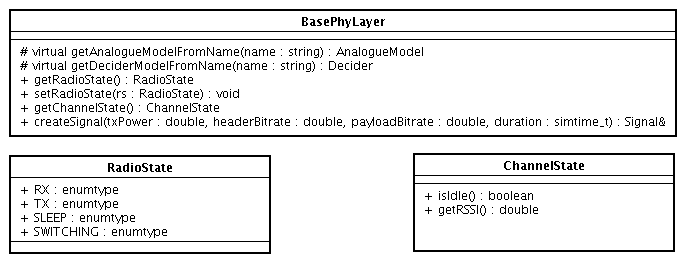
\includegraphics[width = \textwidth]{modelling/BasePhyLayer_members.png}
 \caption{BasePhyLayer interface}
 \label{fig: BasePhyLayer interface}
\end{figure}



\subsection{AnalogueModel}
%\label{AM and Signal}

%The Signal is designed one-dimensional (power-over-time) by default with a
%specified time point for start and end of the Signal. The owner is able
%to add and request values at a specific time point\req{sendInfoTXPower}.
%The Method getTimeIterator() returns an appropriate SignalTimeIterator needed
%for applying AnalogueModels to the Signal.

%\begin{quote}
%\emph{NOTE: Anyone who subclasses Signal should make shure to have a properly
%working SignalTimeIterator (subclassed) for it. The SignalTimeIterator should
%always iterate over every time stamp in each dimension. This way simple
%AnalogueModels will be able to filter the Signal independent from its
%dimension.}
%\end{quote}

%Further the Signal is set the packets bitrate over time\req{sendInfoBitrate}, 
%the Move of the Host\req{sendInfoMove}, the size of the
%packet\req{sendInfoSize} and the channel dimensions\req{sendInfoChannel} by
%\h{\bp}.
%
%\emph{See also \ref{AirFrame and Signal}.}

The AnalogueModel is at least able to filter the \emph{TX-Power over time}-Signal.\\

Information how it works on a more complex multi-dimensional Signal are
explained in section \ref{sec:signaldetail}.
 
\begin{figure}[H]
 \centering
 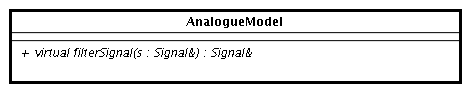
\includegraphics[width = \textwidth]{modelling/AnalogueModel_members.png}
 \caption{analogue model interface}
 \label{fig: analogue model interface}
\end{figure}
%
%The AnalogueModel offers functionality to filter a referenced
%signal\req{analogueFilter} in a specified interval\req{rcvFilterSignals} (e.g.
%preamble\req{rcvFilterPreamble}) or at a single point in time.

%Three basic AnalogueModel classes are foreseen to be plugged into Phy-Layer to
%simulate pathloss\req{analogueSimPathloss}, shadowing\req{analogueSimShadowing}
%and fading\req{analogueSimFading}.\\
%\h{\bp} is designed to apply an arbitrary number of AnalogueModels to a Signal.

% \begin{figure}[H]
%  \centering
%  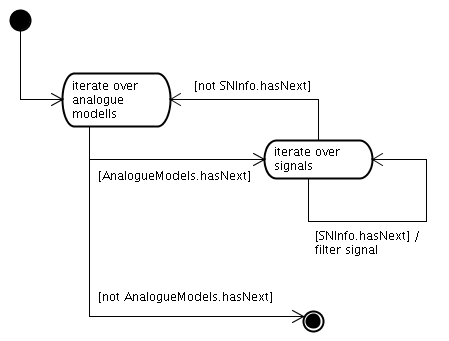
\includegraphics[width =
%0.8\textwidth]{modelling/apply_analogue_modells_detail.png}%[width=300pt]
%  \caption{application of analogue models}
%  \label{fig: application analogue models}
% \end{figure}



\subsection{ChannelInfo}

ChannelInfo keeps track of all AirFrames on the channel. It does not
differentiate between \textit{signal} and \textit{noise}. \h{\bp} is able to
add and remove references to certain AirFrames to and from ChannelInfo.\\
ChannelInfo can return a vector of Signals (references) that intersect with a
given time interval.

\begin{figure}[H]
 \centering
 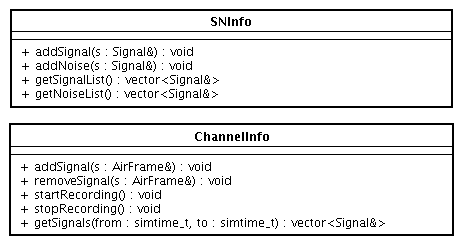
\includegraphics[width = \textwidth]{modelling/ChannelInfo_members.png}
 \caption{channel details}
 \label{fig: channel details}
\end{figure}


\subsection{Decider and DeciderToPhy interface}
\label{decider}

The main task of the Decider is to decide which packets should be handed up to
the MAC layer. To achieve this the \h{\bp} hands every receiving AirFrame
several times to the ``processSignal()``- function of the Decider.

\label{ProcessSignal}
The most common case how a Decider would process AirFrames would be the
following:

\begin{enumerate}
 \item If the Decider gets an AirFrame for the first time, it determines the
time point it can decide if the packet is noise or not and returns this time
point to the \h{\bp}. The time point could be the preamble length, for example.

 \item The next time the Decider gets the packet it would internally decide if
the packet has to be considered noise or not. If the decision is noise the
packet isn't interesting anymore for the Decider. If the packet is classified
as a signal the Decider would return the end of the signal to the \h{\bp}.

 \item When the receiving of the AirFrame is over and the AirFrame wasn't
classified as noise, the Decider would decide if the packet was received
correctly. If the result is positive the Decider has to tell the \h{\bp} to
send the AirFrame together with the DeciderResult to the \h{\bm}.
\end{enumerate}

A second task of the decider is to decide if the channel is busy or idle at a
specific point in time or during a given interval.\\

Since the Decider is responsible to decide if an AirFrame should be
decapsulated and handed up to the MAC layer the Decider needs an interface to
the \h{\bp}.\\

Over the interface the Decider can do the following things:

\begin{itemize}
 \item get the current simulation time
 \item get the list of AirFrames which intersect which a specific interval (to
calculate SNR)
 \item tell the \h{\bp} to hand an AirFrame up to the MAC layer
 \item tell the \h{\bp} to send a control message to the MAC layer
\end{itemize}

Due to the last point the Decider is able to answer a ChannelSenseRequest of the
MAC layer.\\

A Decider that gives a more detailed DeciderResult (e.g. bitwise
errors\req{defdeciderBitwise}) must be subclassed and implemented by the user.

\begin{figure}[H]
 \centering
 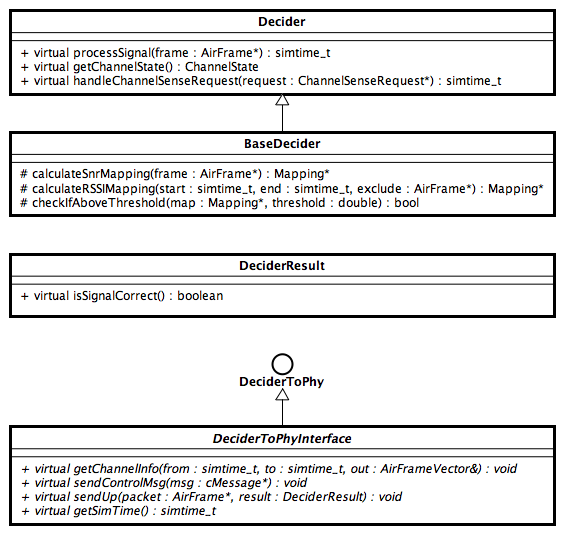
\includegraphics[width = \textwidth]{modelling/DeciderModule_members.png}
 \caption{Decider interface}
 \label{fig: Decider interface}
\end{figure}

\newpage

\subsection{The one-dimensional Signal and AirFrame}
\label{AirFrame and Signal}

AirFrame and Signal both hold information about the packet to send. While the
AirFrame is responsible for the OMNeT related data which is necessary to send
OMNeT messages, the Signal holds the data which is necessary for the simulation
of the transmission process.\\

Here we focus on the basic, one-dimensional (time) Signal that stores entries
for TX Power and attenuation over time\footnote{The time stamps are values
relative to starting time point}. There are fix entries for header and
payload bitrate. These assumptions are considered to cover most cases.
It is possible to obtain a time iterator for this Signal to have access to
entries at specific time points.

Further Signal stores the Move (move pattern of the sending host), the packets
header length, the start time and length of the Signal.\\

\emph{Note: The multi-dimensional Signal is an instance of the same class but
has more functionality. It is described in detail in a separate section.}\\

To be able to control the sending process\req{defsendControl} of an AirFrame
every AirFrame has a unique id and a specific type which specifies if this is a
normal AirFrame or a control-AirFrame. Further it holds an instance of Signal
which represents the physical signal.


\begin{figure}[H]
 \centering
 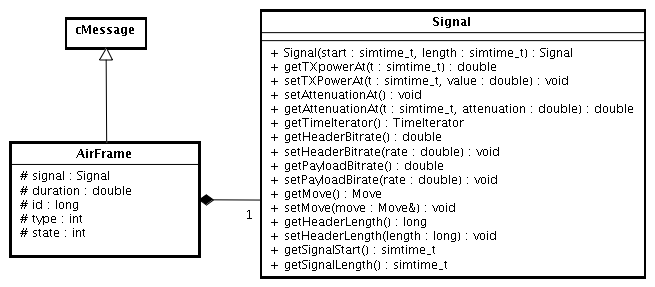
\includegraphics[width = \textwidth]{modelling/AirFrame_members.png}
 \caption{member arrangement in AirFrame and Signal}
 \label{fig:memberAirFrame}
\end{figure}
\newpage

\subsection{receiving a MacPkt}

On reception of a MacPkt from the MAC layer, \h{\bp} checks if:
\begin{enumerate}
	\item the radio is in TX state\req{defsendPreqMode},
	\item it is not already sending a packet\req{defsendPreqSending} 
\end{enumerate} 

If one of these conditions is not fulfilled it will throw an error.\\

The MacToPhyControlInfo object attached to the MacPkt contains the information
needed by \h{\bp} when constructing the AirFrame to send to the channel.
Right now it only contains the Signal initialized by the \h{\bm}.

See \ref{SignalCreation} for how the Signal is created by the \h{\bm}.

\begin{figure}[H]
 \centering
 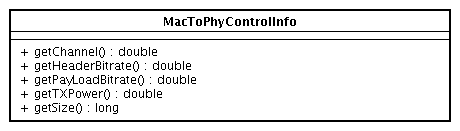
\includegraphics[width = \textwidth]{modelling/MacToPhyCtrlInfo_members.png}
 \caption{MacToPhyControlInfo interface}
 \label{fig: MacToPhyCtrlInfo interface}
\end{figure}


\h{\bp} adds further information to the Signal and is responsible for creating
and initializing the AirFrame and attaching the Signal to it.
For detailed arrangement of information in Signal and AirFrame see \ref{AirFrame
and Signal}.
When the AirFrame is complete and sent, \h{\bp} schedules a TX\_OVER message to
the \h{\bm} (via control-message).

\begin{figure}[H]
 \centering
 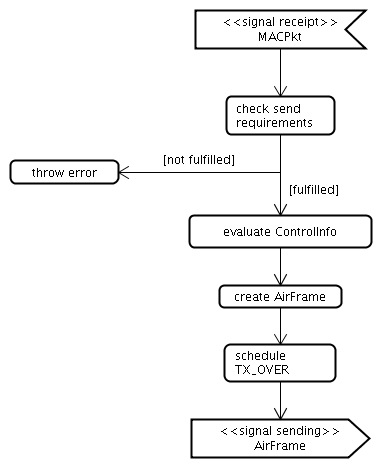
\includegraphics[width = 0.8\textwidth]{modelling/onMACPkt.png}
 \caption{sending process}
 \label{fig: sending process}
\end{figure}
\newpage



\subsection{Receiving and processing an AirFrame}

On arrival of an AirFrame \h{\bp}:
\begin{enumerate}
	
	\item applies AnalogueModels to the corresponding
Signal\req{defrcvSimAttenuation},
	\item receives the AirFrame\req{defrcvSimDuration}.
\end{enumerate}

\begin{figure}[H]
 \centering
 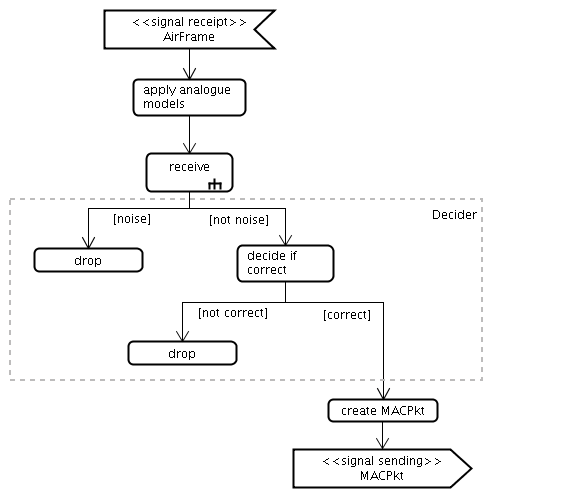
\includegraphics[width = \textwidth]{modelling/onAirFrame.png}
 \caption{receiving process}
 \label{fig: receiving process}
\end{figure}


The receiving process works as follows: In general, time intervals during
reception are simulated by scheduling the AirFrame accordingly.\\

\textbf{stage 0:}\\
An optional propagation delay is simulated by updating the starting time of the
Signal\req{defrcvSimDelay} according to the delay and scheduling the AirFrame to
the reception start point.\\

\textbf{stage 1:}\\
On reception start the Signal is given to the Decider for processing. The
Decider returns a time point it wants to process the Signal again.
This time point has to be before the end of the Signal otherwise an error
is thrown. \\

\textbf{stage 2:}\\
The AirFrame is scheduled arbitrary times for the Decider processing method
until it either returns a negative time point or the time point of the end of
the
Signal. In both cases the state is increased by one before the AirFrame is
scheduled to its end. See \ref{ProcessSignal} for more details on the Deciders
Signal processing. \\

\textbf{stage 3:}\\
Finally reception is over and the AirFrame is completely received in reality.

\emph{Note: The Decider process is responsible for telling the \h{\bp} to send
a MacPkt to the \h{\bm}.}

\begin{figure}[H]
 \centering
 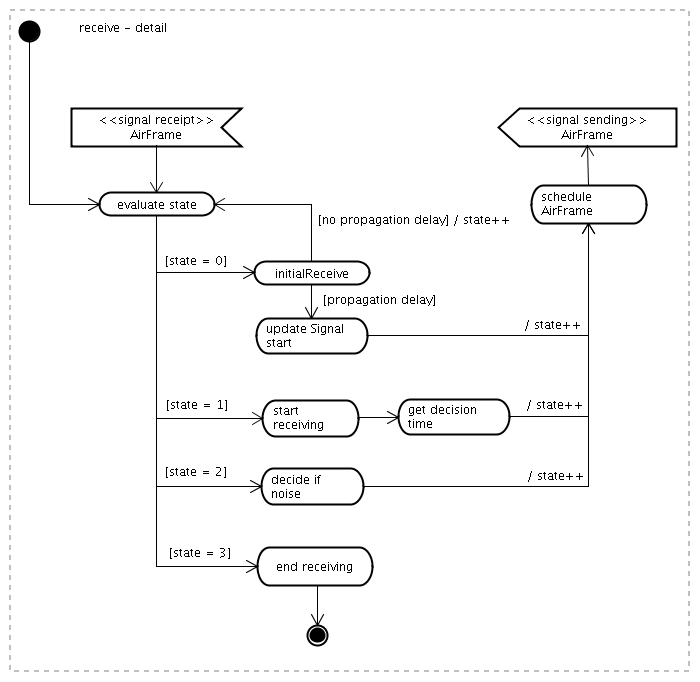
\includegraphics[width = \textwidth]{modelling/receive_detail.png}
 \caption{receive detail}
 \label{fig: receive detail}
\end{figure}


% The receiving process is modelled internally by a state machine that schedules
%the AirFrame that is received (since we have a pointer to it from the
%beginning) everytime a delay/time interval shall be simulated. That saves us
%the creation of additional self-messages.




%When the preamble of a packet is completely received, \h{\bp} constructs a
%SNInfo for the preamble, applies the AnalogueModels to it and passes it to the
%Decider to find out whether this packet is considered noise.

%\begin{figure}[H]
% \centering
% 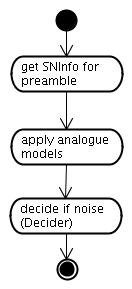
\includegraphics[width = 0.2\textwidth]{modelling/end_preamble_detail.png}
% \caption{end preamble detail}
% \label{fig: end preamble detail}
%\end{figure}

%In case a received packet is not \textit{noise} it is processed, i.e. \h{\bp}
%creates the corresponding SNInfo for the packet, applies AnalogueModels to it
%and passes the result to the Decider to check whether the packet was received
%correctly. If so, a MacPkt is created and handed up to
%Phy-Layer\req{defrcvPassToMAC}.


\subsection{the .ned-file}

The .ned-file of the \h{\bp} has the following parameters:

\begin{itemize}
\item usePropagationDelay as \textit{boolean}\req{defconfDelay}
\item analogueModels as
\textit{XML}\req{defconfAnalogue}\req{defconfAnalogueParam}
\item decider as \textit{XML}\req{defconfDecider}\req{defconfDeciderParam}
\item thermalNoise as \textit{numeric const}\req{defconfNoise}
\item sensitivity as \textit{numeric const}\req{defconfSens}
\item maximal TX power as \textit{numeric const}\req{defconfMaxTXPower}
\item switchTimeRX as \textit{numeric const}\req{defconfSwitchingTimes}
\item switchTimeTX as \textit{numeric const}\req{defconfSwitchingTimes}
\item switchTimeSleep as as \textit{numeric const}\req{defconfSwitchingTimes}
\end{itemize}

The parameters "analogueModels" and "decider" store which AnalogueModels and
which Decider are to be used, together with their parameters in XML format. The
exact format still has to be declared!

%\subsection{provide status information to MAC}

%Passively provided information\req{defprovpassive}: \h{\bm} is equipped with a
%reference to \h{\bp} in order to obtain information
%about channelstate\req{defchannelstate} and current radio
%state\req{defcurrentmode}
%by
%simple method calls. \\
%Actively provided information\req{defprovactive}: A cMessage of the kind
%TX\_OVER
%is sent to MAC layer when a sending transmission is over\req{deftxover},
%\saf{sending process}.



%\subsection{send packets}

%Since \h{\bm} has a reference to \h{\bp} it can obtain information about the
%state the radio is is currently in\req{defsendPreqMode}, it is not already
%sending
%to the channel on its own\req{defsendPreqSending} and the channel is
%idle\req{defsendPreqIdle} via method calls, \saf{BasePhyLayer interface}.

%The class MacToPhyControlInfo is designed as the container for control
%info\req{defpacketFromMac} the MAC layer
%wants to attach to the packet given down to Phy-Layer for sending.
%The packet itself is handed down as a MacPkt via OMNeT-channel. 



\subsection{signal details}
\label{sec:signaldetail}

The Signal class should be able to support multiple dimensions for arguments (time, channel, space, ...) and values (TX power, attenuation, bitrate). That means both sides of our signal function have to be extendable.

The following section explains how we achieve this.

\subsubsection{multiple dimensions for values}

Generally spoken a function can be implemented as a map from ``Argument`` to
''Value``. With inheritance we could basically use everything as a Value.
If we assume that every Value of our Signals is in $\mathbb{R}^n$ we could
implement it as a vector of doubles of size \textit{n}.

\subsubsection{multiple dimensions for arguments}

While we could use basically everything as Value the Argument has to be
distinguishable. Further a simple map with an Argument class as key would be
hard to iterate reasonable and fast.

So instead of using one map from Argument to Value we realize multiple
dimensions by using sub signals (see figure \ref{fig:signalscheme}). We add a
dimension of arguments by implementing a map from the argument value to another
sub-signal. This structure has three advantages:

\begin{enumerate}
\item The Signal dimensions are easy to extend.
\item It provides a deterministic way to iterate over it.
\item And if every sub signal knows its dimension we can still use an Argument class (which would be, same as the Value, an extendable vector of doubles) for direct access to a specific Value of the Signal.
\end{enumerate}


\begin{figure}[H]
 \centering
 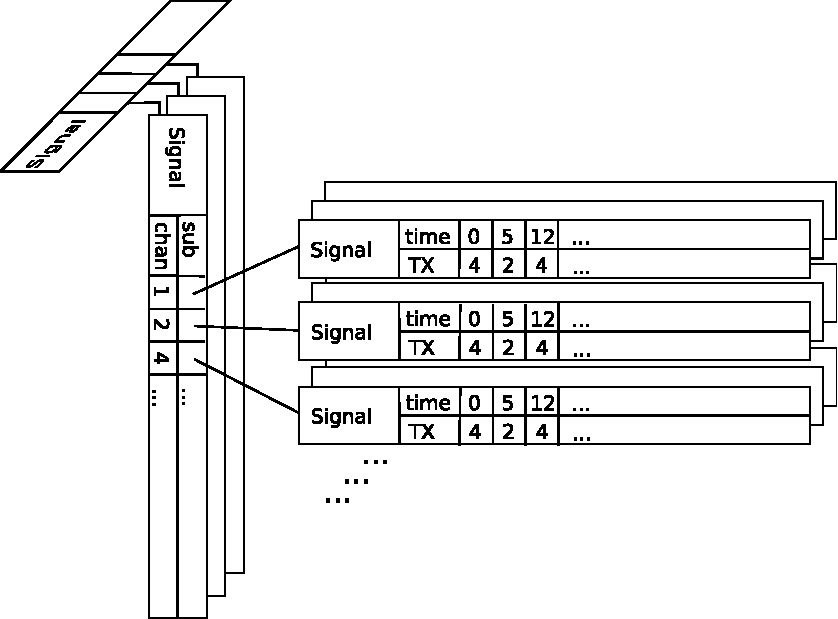
\includegraphics[width = 0.8\textwidth]{SignalDetail/signal_scheme.pdf}
 \caption{multi dimensional signals}
 \label{fig:signalscheme}
\end{figure}

\subsubsection{creating and identifying Signals}

Three things have to be considered:

\begin{enumerate}
\item We have three classes now (Signal, Argument and Value) which depends all on the type (meaning the dimensions) of the Signal. So we have to make sure to create the appropriate Arguments and Values for a Signal.
\item A receiving physical layer could receive different types of Signals during runtime, so we need a way to identify the type of a Signal.
\item The Signal types have to be globally known by each Physical Layer in the simulation.
\end{enumerate}

We solve the first two problems by introducing a SignalPrototype class. If we want to create a new Signal type we create a new SignalPrototype with the parameters for the Signal type (which would be the dimensions). The SignalPrototype then is able to create the appropriate Signals, Arguments and Values. It is also used as Identifier for the Signal type.

The last problem is solved by a simulation wide known SignalDatabase which maps 
a Signal type name ("MIMO signal" for example) to the associated Prototype.
Every new SignalPrototype has to be registered by a unique name with the
SignalDatabase. 

\subsubsection{detailed class diagram of Signal}

The above decisions lead to the following class diagram:

\begin{figure}[H]
 \centering
 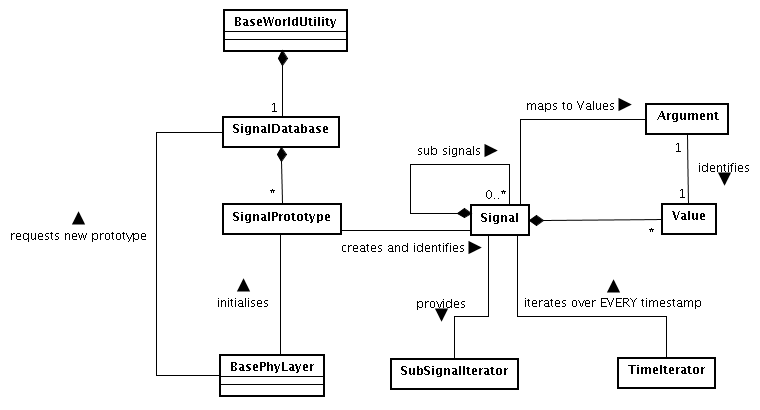
\includegraphics[width = \textwidth]{SignalDetail/class_diagram.png}
 \caption{detailed class diagram}
 \label{fig: signal classgraph}
\end{figure}

\newpage
\subsubsection{creation of new signal types}

To assure that every new SignalPrototype is registered with the database we
don't provide a public constructor for the SignalPrototype. If a physical layer
wants to create a new prototype it has to ask the database if a prototype with
the same name is already registered. If not it can ask the database to create a
new one with the given name.\\

We assume that every Signal has at least time as argument dimension and TX 
power and attenuation as value dimensions. So these dimensions are already
included in every new prototype.

Additional dimensions have to be registered by name with the prototype. The 
registration methods returns a unique sequential number for the registered
dimension. This number is used later as a fast way to access the values of the
dimension.

If every dimension is registered at the prototype one can create proper new 
Signals, Arguments and Values with this SignalPrototype.\\

\emph{Note: The first time the SignalPrototype is used to create a Signal, 
Argument or Value it is internally locked and no other dimensions can be
registered.}\\

The "isPrototypeFor()" method can be used to check if a Signal was created by 
this Prototype.

\begin{figure}[H]
 \centering
 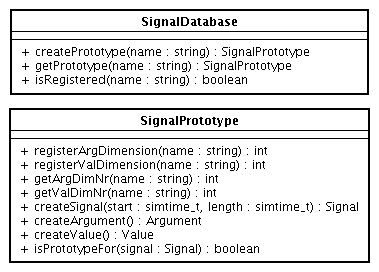
\includegraphics[width =  0.8\textwidth]{SignalDetail/database_members.png}
 \caption{interface of Database and Prototype}
 \label{fig: Database members}
\end{figure}
\newpage
\subsubsection{accessing the Signal}

The following class diagram shows the methods which the Signal provides
\textbf{additionally} to those listed in figure \ref{fig:memberAirFrame}.

\begin{figure}[H]
 \centering
 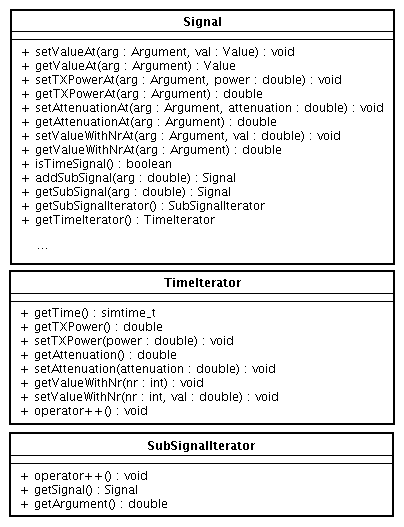
\includegraphics[width =  0.8\textwidth]{SignalDetail/signal_members.png}
 \caption{signal interface details}
 \label{fig: detailed signal members}
\end{figure}

The TimeIterator still iterates over every time stamp of the Signal, independent
from the dimension of the Signal. This way simple filters can be applied without
knowledge of the exact type of the Signal.\\

The easiest way to access a specific value of the Signal, is to create an 
instance of the apropriate Argument (and Value, if you want to change it),
initialize its dimensions with the wanted values and then use the "getValueAt()"
and "setValueAt()" methods. Here one has to know that an entry for the given
Argument actually exists, otherwise the Signal would have to interpolate the
Value.\\

The SubSignalIterator can be used to iterate recursively over every pair of 
value and its associated sub signal of the dimension this Signal represents. The
deepest SubSignal will always be the time dimension which can be checked by
"isTimeSignal()".

\begin{figure}[H]
 \centering
 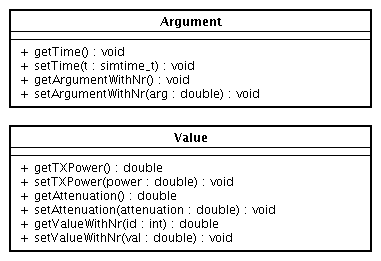
\includegraphics[width =  0.8\textwidth]{SignalDetail/argval_members.png}
 \caption{interface for Argument and Value}
 \label{fig: arg and val members}
\end{figure}

The SignalPrototype associates every argument dimension name with a unique 
sequential number. The same holds for the value dimensions. These numbers can be
used to access the values in Argument or Value with the 
"get*WithNr()" methods.

Because every Argument has a time dimension and every Value a TX power and an 
attenuation, the classes provide short cuts to these values.

%\section{Appendix}

\begin{figure}[h]
 \centering
 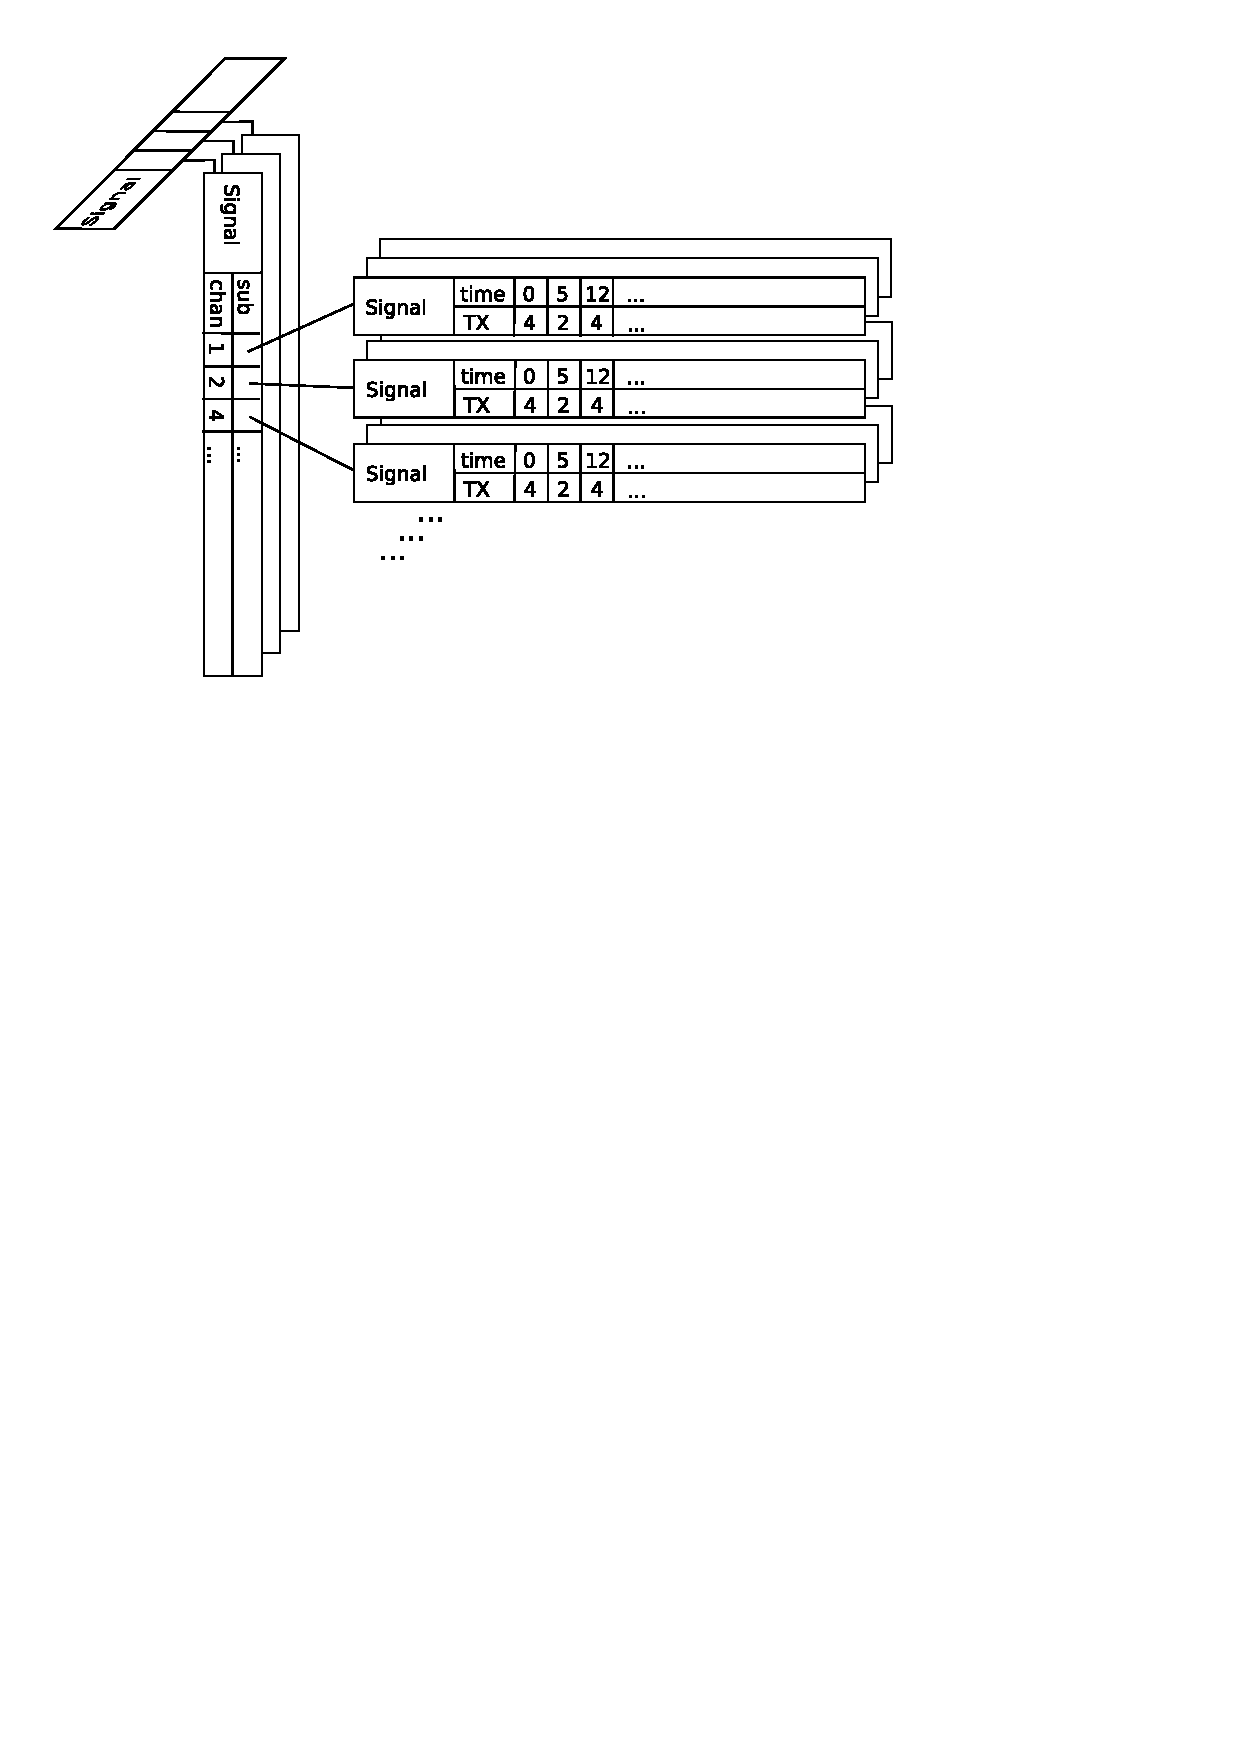
\includegraphics[width=400pt]{signal/signal.pdf}
 \caption{class graph}
 \label{fig: signal abstract}
\end{figure}

%\begin{figure}[h]
% \centering
% 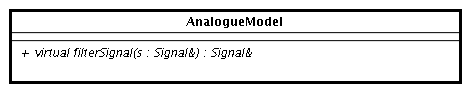
\includegraphics[width=340pt]{modelling/AnalogueModel_members.png}
% \caption{analogue model interface}
% \label{fig: analogue model interface}
%\end{figure}

%\begin{figure}[h]
% \centering
% 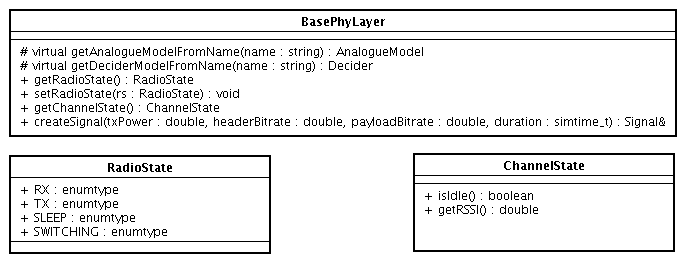
\includegraphics[width=340pt]{modelling/BasePhyLayer_members.png}
% \caption{BasePhyLayer interface}
% \label{fig: BasePhyLayer interface}
%\end{figure}

%\begin{figure}[h]
% \centering
% 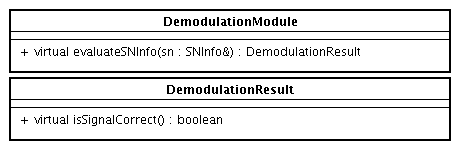
\includegraphics[width=340pt]{modelling/DemodulationModule_members.png}
% \caption{Demodulator interface}
% \label{fig: Demodulator interface}
%\end{figure}

%\begin{figure}[h]
% \centering
% 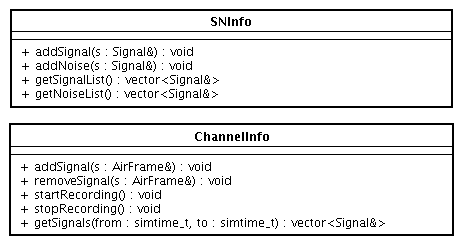
\includegraphics[width=340pt]{modelling/ChannelInfo_members.png}
% \caption{channel details}
% \label{fig: channel details}
%\end{figure}

%\begin{figure}[h]
% \centering
% 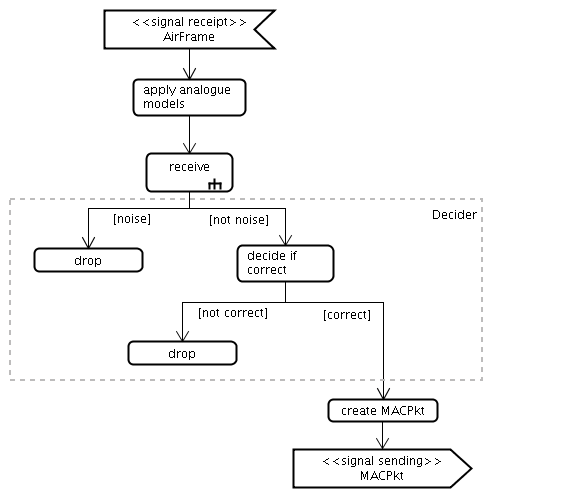
\includegraphics[width=340pt]{modelling/onAirFrame.png}
% \caption{receiving process}
% \label{fig: receiving process}
%\end{figure}

%\begin{figure}[h]
% \centering
% 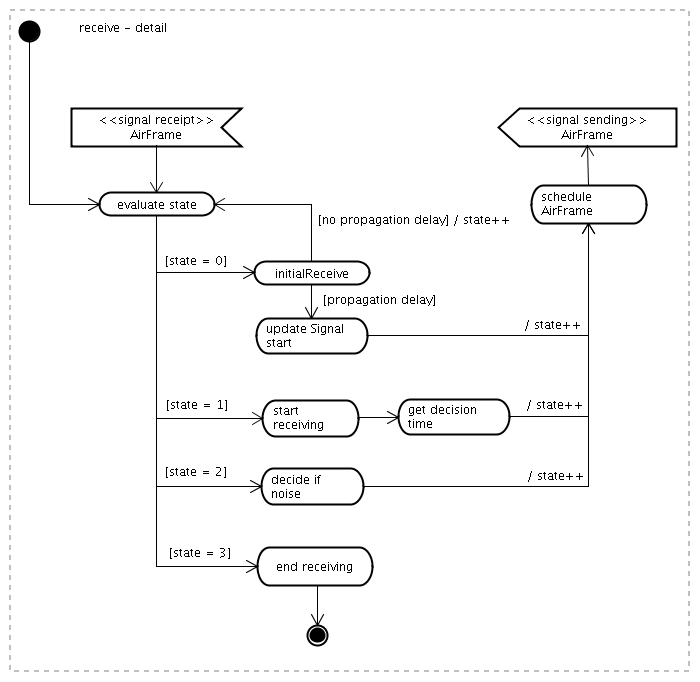
\includegraphics[width=340pt]{modelling/receive_detail.png}
% \caption{receive detail}
% \label{fig: receive detail}
%\end{figure}

%\begin{figure}[h]
% \centering
% 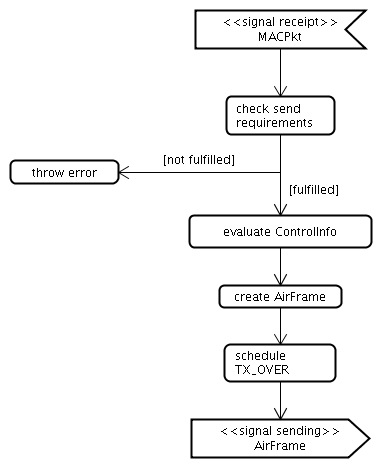
\includegraphics[width=300pt]{modelling/onMACPkt.png}
% \caption{sending process}
% \label{fig: sending process}
%\end{figure}


\end{document}
